\documentclass[11pt]{article}
\usepackage[margin=1in]{geometry}
\usepackage{amsmath,amssymb,amsthm}
\usepackage{graphicx,booktabs}
\usepackage[colorlinks=true,linkcolor=blue,citecolor=blue,urlcolor=blue]{hyperref}

\newtheorem{proposition}{Proposition}
\newtheorem{lemma}{Lemma}
\newtheorem{corollary}{Corollary}
\theoremstyle{definition}
\newtheorem{definition}{Definition}
\theoremstyle{remark}
\newtheorem{remark}{Remark}

\newcommand{\E}{\mathbb{E}}
\newcommand{\qbar}{\bar q}
\newcommand{\VPI}{\mathrm{VPI}}
\newcommand{\gcav}{\hat g}
\newcommand{\cL}{\mathcal{L}}
\newcommand{\cR}{\mathcal{R}}
\newcommand{\ind}[1]{\mathbf{1}_{#1}}
\DeclareMathOperator{\Var}{Var}

\title{The Learning Premium in the Large-Horizon Limit\\[3pt]
\large Propositions 1--2 (draft for \emph{Orchestrating Agent Teams})}
\author{Working draft}
\date{\today}

\begin{document}
\maketitle

\begin{abstract}
We show that, as the campaign horizon $K$ grows with the budget per period $\rho=B/K$ held fixed,
the per-period learning premium of the learn-then-exploit (ETC) team converges to an explicit function
of the primitives: the value of the best binomial probing experiment, which coincides with the value of
free perfect information $\VPI(\rho)$ outside a neighbourhood of the entry threshold. The limit does not depend on
how the team schedules its learning, so the direction of the planner's reallocation in the limit is
pinned down by primitives alone (Proposition~\ref{prop:limit} and Corollary~\ref{cor:alloc}). We then
characterise the shape of the limit premium (Proposition~\ref{prop:shape}): it is negative-to-zero at small
budgets (information, even if free, lowers the value of a budget-paced team), positive and decaying like
$\Var(\theta)/\rho^2$ at large budgets, and it opens with a kink, so the marginal-value ratio jumps at entry.
The upper edge of the learning window is a finite-horizon effect.
\end{abstract}

\section{Setup and notation}\label{sec:setup}

We keep the model of the paper. The market state is $\theta\in\{\theta_L,\theta_H\}$ with $0<\theta_L<\theta_H$
and prior $\pi_0=\Pr(\theta=\theta_H)\in(0,1)$; $r=\theta_H/\theta_L$, $b^I=\sqrt{\theta_L\theta_H}$ and
$\kappa_0=\pi_0/(1-\pi_0)$. A bid $b$ wins with probability $q_\theta(b)=b/(b+\theta)$ and pays $b$ upon winning;
$\qbar(\pi,b)=\pi q_{\theta_H}(b)+(1-\pi)q_{\theta_L}(b)$. A team has budget $B$ and horizon $K$; we write
$\rho=B/K$ for the budget per period and index values by $K$ when the horizon matters.

\paragraph{Budget accounting and the rate function.} As in the paper, whenever a team commits to an
exploitation plan at belief $\pi$ with remaining budget $R$ over $n$ periods, the plan spends $R$ in
expectation under $\pi$. By Lemma~2 of the paper (Exploitation phase) the optimal plan is a constant paced bid and
its value is $n\,g(\pi;R/n)$, where for $\pi\in[0,1]$ and $\rho\ge0$
\begin{equation}\label{eq:g}
g(\pi;\rho):=\qbar\bigl(\pi,b^*(\pi,\rho)\bigr),\qquad b^*(\pi,\rho)\,\qbar\bigl(\pi,b^*(\pi,\rho)\bigr)=\rho .
\end{equation}
In particular the no-learning benchmark is $W_K(B)=K\,g(\pi_0;B/K)$.

\paragraph{Learn-then-commit protocols.} A protocol in the class $\cL$ probes at a fixed bid $b_p>0$ for $\sigma$
periods, where $\sigma\le K-1$ is a stopping time of the probe outcomes, and hands the number of wins
$w_\sigma$ to an exploitation agent that commits at the posterior $\pi_\sigma$ to the paced plan with the remaining
budget $R_\sigma=B-w_\sigma b_p\ge0$ over the remaining $K-\sigma$ periods. By Lemma~2 of the paper its value is
\begin{equation}\label{eq:VL}
V_K^{\sigma}(B)=\E\Bigl[w_\sigma+(K-\sigma)\,g\Bigl(\pi_\sigma;\frac{R_\sigma}{K-\sigma}\Bigr)\Bigr].
\end{equation}
The paper's ETC is the case $b_p=b^I$ and $\sigma\equiv\tau$ deterministic, with
$V_K(B)=\max\{V_K^{\tau}(B):0\le\tau\le\min(K-1,B/b^I)\}$; the adaptive-stopping version (draft DP) is $b_p=b^I$
with $\sigma$ chosen optimally. Expectations are under the prior-predictive law, under which the posterior
$(\pi_t)_t$ is a martingale with $\E[\pi_t]=\pi_0$.

\begin{definition}[Limit objects]\label{def:limit}
For $\rho>0$ let $\pi_\tau$ denote the posterior after $\tau$ probes at $b^I$ and $\pi_\infty:=\ind{\{\theta=\theta_H\}}$. Define
\begin{align*}
\VPI(\rho)&:=\pi_0\,g(1;\rho)+(1-\pi_0)\,g(0;\rho)-g(\pi_0;\rho),\\
f_\tau(\rho)&:=\E\bigl[g(\pi_\tau;\rho)\bigr]-g(\pi_0;\rho)\quad(\tau\in\mathbb N),\qquad f_\infty:=\VPI,\\
\Psi(\rho)&:=\max\Bigl\{0,\ \sup_{\tau\in\mathbb N\cup\{\infty\}} f_\tau(\rho)\Bigr\},\\
\Phi(\rho)&:=\gcav(\pi_0;\rho)-g(\pi_0;\rho),
\end{align*}
where $\gcav(\cdot;\rho)$ is the concave envelope of $g(\cdot;\rho)$ on $[0,1]$. Thus $\VPI$ is the per-period value
of free perfect information, $\Psi$ the value of the best binomial probing experiment at $b^I$ (including none), and
$\Phi$ the value of the best information structure. Since $\E[\pi_\tau]=\pi_0$ and
$\gcav$ is concave, $\max\{\VPI(\rho),0\}\le\Psi(\rho)\le\Phi(\rho)$.
\end{definition}

\begin{lemma}[Properties of $g$]\label{lem:g}
\begin{enumerate}
\item[(i)] For every $\pi$, $\rho\mapsto g(\pi;\rho)$ is continuous, strictly increasing and strictly concave on
$[0,\infty)$, with $g(\pi;0)=0$ and $g<1$.
\item[(ii)] For every $\pi$ and $S\ge0$, $n\mapsto n\,g(\pi;S/n)$ is nondecreasing on $(0,\infty)$.
\item[(iii)] For $\rho>0$, $g(\cdot;\rho)\in C^\infty([0,1])$, and $g$, $\partial_\pi g$, $\partial_\rho g$ are bounded on
$[0,1]\times[\rho_a,\rho_b]$ for every $0<\rho_a<\rho_b<\infty$.
\end{enumerate}
\end{lemma}

\begin{proof}
(i) is shown in the proof of Lemma~2 of the paper. (ii) Concavity and $g(\pi;0)=0$ imply that
$x\mapsto g(\pi;x)/x$ is nonincreasing on $(0,\infty)$; hence $n\,g(\pi;S/n)=S\cdot g(\pi;S/n)/(S/n)$ is
nondecreasing in $n$. (iii) $F(b,\pi,\rho)=b\,\qbar(\pi,b)-\rho$ is rational in $(b,\pi)$ with positive
denominators and $\partial_bF=\qbar+b\,\partial_b\qbar>0$ for $b>0$; the implicit function theorem gives a
$C^\infty$ solution $b^*(\pi,\rho)$ for $\rho>0$, and boundedness follows from continuity on compact sets.
\end{proof}

\begin{lemma}[Posterior concentration at $b^I$]\label{lem:conc}
Let $\beta:=2r^{1/4}/(1+\sqrt r)\in(0,1)$, the Bhattacharyya coefficient of the two outcome distributions at
$b^I$. For every $\tau\in\mathbb N$,
$\E\bigl[|\pi_\tau-\pi_\infty|\bigr]\le 2\sqrt{\pi_0(1-\pi_0)}\;\beta^{\tau}$.
\end{lemma}

\begin{proof}
At $b^I$ the win probabilities are $p_H=1/(1+\sqrt r)$ and $p_L=\sqrt r/(1+\sqrt r)$, and the posterior odds are
$\kappa_\tau=\kappa_0r^{(\tau-2w)/2}$. Under $\theta_H$, $1-\pi_\tau=1/(1+\kappa_\tau)\le\kappa_\tau^{-1/2}$ and each
probe multiplies $\kappa^{-1/2}$ by $r^{1/4}$ (win) or $r^{-1/4}$ (loss), so
$\E[1-\pi_\tau\mid\theta_H]\le\kappa_0^{-1/2}\bigl(p_Hr^{1/4}+(1-p_H)r^{-1/4}\bigr)^{\tau}=\kappa_0^{-1/2}\beta^{\tau}$.
Symmetrically $\E[\pi_\tau\mid\theta_L]\le\kappa_0^{1/2}\beta^\tau$. Averaging with weights $\pi_0,1-\pi_0$ gives
the bound. Finally $\beta<1$ because $1+\sqrt r>2r^{1/4}$ for $r\neq1$.
\end{proof}

\section{Proposition 1: the large-horizon limit}\label{sec:prop1}

\begin{proposition}[Large-horizon limit of the learning premium]\label{prop:limit}
Fix $\rho>0$ and let $B=\rho K$.
\begin{enumerate}
\item[(a)] \emph{Achievability.} There are constants $c_\rho,c'_\rho$ (depending on the primitives and $\rho$ only)
such that for every $\tau\in\mathbb N$ and all $K$ large enough
\[
\frac{V_K^{\tau}(\rho K)-W_K(\rho K)}{K}\ \ge\ f_\tau(\rho)-c_\rho\frac{\tau}{K},
\]
and for $\tau_K=\lceil\log K/\log(1/\beta)\rceil$,
\[
\frac{V_K^{\tau_K}(\rho K)-W_K(\rho K)}{K}\ \ge\ \VPI(\rho)-c'_\rho\,\frac{1+\log K}{K}.
\]
Consequently $\liminf_{K}\,[V_K(\rho K)-W_K(\rho K)]/K\ge\Psi(\rho)$.
\item[(b)] \emph{Upper bound.} For every protocol in $\cL$ and every $K,B$,
\[
\frac{V^{\sigma}_K(B)-W_K(B)}{K}\ \le\ \frac{\E[\sigma]}{K}+\Phi(B/K),
\]
and for the paper's ETC with a deterministic $\tau$, $[V^{\tau}_K(B)-W_K(B)]/K\le\tau/K+\Psi(B/K)$.
\item[(c)] \emph{Limit.} The optimal probing length satisfies $\tau^*_K/K\to0$, and
\[
\lim_{K\to\infty}\frac{V_K(\rho K)-W_K(\rho K)}{K}=\Psi(\rho).
\]
\item[(d)] \emph{Protocol invariance.} For every sequence of protocols in $\cL$ with $\E[\sigma_K]=o(K)$,
\[
\limsup_K\ [V^{\sigma_K}_K(\rho K)-W_K(\rho K)]/K\ \le\ \Phi(\rho).
\] On the set
$\cR:=\{\rho:\Phi(\rho)=\max\{\VPI(\rho),0\}\}$ the paper's ETC is asymptotically optimal in this class, and its
limit premium $\max\{\VPI(\rho),0\}$ depends on the primitives $(\theta_L,\theta_H,\pi_0)$ only.
\end{enumerate}
\end{proposition}

\begin{proof}
\emph{(a)} Fix $\tau$; for $K$ large, $\tau\le K-1$ and $\tau b^I\le\rho K$, so $\tau$ is feasible. Since $w\le\tau$,
the exploitation budget per period satisfies
$R/(K-\tau)\ge\rho_K^\tau:=\rho-\tau b^I/(K-\tau)\ge\rho/2$. Dropping the probe wins in \eqref{eq:VL} and using
monotonicity and the Lipschitz bound $L_\rho:=\sup\{\partial_\rho g(\pi;x):\pi\in[0,1],x\in[\rho/2,\rho]\}$ from
Lemma~\ref{lem:g}(iii),
\[
V_K^\tau(\rho K)\ge(K-\tau)\,\E\bigl[g(\pi_\tau;\rho_K^\tau)\bigr]
\ge(K-\tau)\,\E\bigl[g(\pi_\tau;\rho)\bigr]-L_\rho\tau b^I
\ge K\,\E\bigl[g(\pi_\tau;\rho)\bigr]-\tau(1+L_\rho b^I),
\]
using $g<1$. Subtracting $W_K(\rho K)=K g(\pi_0;\rho)$ gives the first bound with $c_\rho=1+L_\rho b^I$. For
$\tau=\tau_K$, the mean value theorem with $M_\rho:=\max_\pi|\partial_\pi g(\pi;\rho)|$ and
Lemma~\ref{lem:conc} give
$f_{\tau_K}(\rho)\ge\VPI(\rho)-2M_\rho\sqrt{\pi_0(1-\pi_0)}\,\beta^{\tau_K}\ge\VPI(\rho)-M_\rho/K$, since
$\beta^{\tau_K}\le1/K$; combining with the first bound and $\tau_K\le1+\log K/\log(1/\beta)$ proves the second.
Since $V_K\ge V_K^\tau$ for every feasible $\tau$, $\liminf_K[V_K-W_K]/K\ge f_\tau(\rho)$ for all
$\tau\in\mathbb N\cup\{\infty\}$, and $\tau=0$ gives $0$; hence the $\liminf$ is at least $\Psi(\rho)$.

\emph{(b)} In \eqref{eq:VL}, $R_\sigma\le B$, monotonicity and Lemma~\ref{lem:g}(ii) give
$(K-\sigma)\,g(\pi_\sigma;R_\sigma/(K-\sigma))\le(K-\sigma)\,g(\pi_\sigma;B/(K-\sigma))\le K\,g(\pi_\sigma;B/K)$,
and $w_\sigma\le\sigma$. By optional stopping $\E[\pi_\sigma]=\pi_0$, so by concavity of $\gcav$,
$\E[g(\pi_\sigma;\rho)]\le\E[\gcav(\pi_\sigma;\rho)]\le\gcav(\pi_0;\rho)$. Hence
$V_K^\sigma(B)\le\E[\sigma]+K\gcav(\pi_0;\rho)$; subtract $W_K(B)=Kg(\pi_0;\rho)$. For deterministic $\tau$ at $b^I$,
replace $\gcav(\pi_0;\rho)$ by $\E[g(\pi_\tau;\rho)]=g(\pi_0;\rho)+f_\tau(\rho)\le g(\pi_0;\rho)+\Psi(\rho)$.

\emph{(c)} Suppose $\limsup_K\tau^*_K/K>0$ and pass to a subsequence with $\tau^*_K/K\to\varepsilon\in(0,1]$.
Feasibility ($\tau b^I\le\rho K$) gives $\varepsilon b^I\le\rho$. Since $\tau^*_K\to\infty$, conditional on $\theta$ the
strong law gives $w/\tau^*_K\to q_\theta(b^I)$ and Lemma~\ref{lem:conc} gives $\pi_{\tau^*_K}\to\pi_\infty$. With
$s_\theta:=b^Iq_\theta(b^I)$, dominated convergence in \eqref{eq:VL} yields
\[
\lim_K\frac{V_K^{\tau^*_K}(\rho K)}{K}=\E_\theta\Bigl[\varepsilon\,q_\theta(b^I)+(1-\varepsilon)\,
g\Bigl(\pi_\infty;\tfrac{\rho-\varepsilon s_\theta}{1-\varepsilon}\Bigr)\Bigr]
\]
(for $\varepsilon=1$ the second term is absent). Because $b^I$ is the paced bid for spend $s_\theta$ in a known state,
$q_\theta(b^I)=g(\pi_\infty;s_\theta)$ on $\{\theta\}$, and strict concavity of $g(\pi_\infty;\cdot)$ gives
$\varepsilon g(\pi_\infty;s_\theta)+(1-\varepsilon)g(\pi_\infty;\frac{\rho-\varepsilon s_\theta}{1-\varepsilon})\le g(\pi_\infty;\rho)$
with equality only if $s_\theta=\rho$ (for $\varepsilon=1$: $g(\pi_\infty;s_\theta)\le g(\pi_\infty;\rho)$ because
$s_\theta<b^I\le\rho$). As $s_{\theta_L}\neq s_{\theta_H}$, the inequality is strict for at least one state, so
$\lim_K V_K^{\tau^*_K}/K<\E_\theta[g(\pi_\infty;\rho)]=g(\pi_0;\rho)+\VPI(\rho)\le g(\pi_0;\rho)+\Psi(\rho)$, which by
(a) is at most $\liminf_K V_K/K$ --- contradicting $V_K=V_K^{\tau^*_K}$. Hence $\tau^*_K=o(K)$, and (b) gives
$\limsup_K[V_K-W_K]/K\le\Psi(\rho)$; together with (a) the limit is $\Psi(\rho)$.

\emph{(d)} The first claim is (b). On $\cR$, $\max\{\VPI,0\}\le\Psi\le\Phi=\max\{\VPI,0\}$, so the ETC limit in (c)
attains the upper bound.
\end{proof}

\begin{corollary}[Allocation in the limit]\label{cor:alloc}
Let $L(\rho):=g(\pi_0;\rho)+\Psi(\rho)$ for $\rho>0$ and $L(0)=0$. Fix $v_1>v_2>0$ and $t>0$, and let $T=tK$. Then
$a^E_K/K=\alpha^E(t):=\arg\max_{\alpha\in[0,t]}\{v_1g(\pi_0;\alpha)+v_2g(\pi_0;t-\alpha)\}$ for every $K$, and every
limit point of $a^L_K/K$ maximizes $v_1L(\alpha)+v_2L(t-\alpha)$ over $\alpha\in[0,t]$. If that maximizer
$\alpha^L(t)$ is unique, $(a^L_K-a^E_K)/K\to\alpha^L(t)-\alpha^E(t)$. At differentiability points and under the
concavity condition of Theorem~1 of the paper, the sign of the limit shift is the sign of
\[
\frac{L'(\alpha^E)}{g_\rho(\pi_0;\alpha^E)}-\frac{L'(t-\alpha^E)}{g_\rho(\pi_0;t-\alpha^E)},
\]
so the direction of the reallocation in the limit is determined by the primitives alone.
\end{corollary}

\begin{proof}
$W_K(\alpha K)=Kg(\pi_0;\alpha)$ makes the benchmark problem independent of $K$. For each $K$,
$\rho\mapsto V_K(\rho K)/K$ is nondecreasing (a larger budget enlarges the feasible set of $\tau$ and raises every
exploitation value) and converges pointwise to $L$ by Proposition~\ref{prop:limit}(c). The family
$\{f_\tau\}$ is equi-Lipschitz on compact subsets of $(0,\infty)$ (Lemma~\ref{lem:g}(iii)), so $\Psi$ is continuous
there, and $\Psi=0$ near $0$ by Proposition~\ref{prop:shape}(a); thus $L$ is continuous on $[0,\infty)$. Pointwise
convergence of monotone functions to a continuous limit on a compact interval is uniform (P\'olya), so the planner's
normalised objectives converge uniformly on $[0,t]$ and limit points of maximisers maximise the limit objective. The
sign statement is Theorem~1 of the paper applied to $L$, noting $W_K'(B)=g_\rho(\pi_0;B/K)$.
\end{proof}

\begin{remark}[Learning while exploiting]
Proposition~\ref{prop:limit} covers every learn-then-commit protocol. A team that updates after every auction and
re-paces its remaining budget (certainty-equivalent pacing, ``CE'') is not in $\cL$. In this model every bid is
informative ($q_{\theta_L}(b)\neq q_{\theta_H}(b)$ for all $b>0$), so such a team learns the state while exploiting,
and the numerical evidence in Section~\ref{sec:numerics} shows that its per-period premium converges to $\VPI(\rho)$ with a learning cost
that grows much more slowly in $K$ than that of fixed-$\tau$ ETC. A proof along the lines of (a) requires posterior concentration under
bids bounded away from $0$ and $\infty$ and control of the realised-wallet re-pacing; we leave it for future work.
\end{remark}

\section{Proposition 2: the shape of the limit premium}\label{sec:prop2}

Let $m_k(\pi):=\pi\theta_H^{-k}+(1-\pi)\theta_L^{-k}$ and $\mu_k(\pi):=\pi\theta_H^{k}+(1-\pi)\theta_L^{k}$ (the $k$-th
moments of $1/\theta$ and $\theta$ under belief $\pi$), and let $\Var_{\pi_0}(\theta)=\pi_0(1-\pi_0)(\theta_H-\theta_L)^2$.

\begin{proposition}[Shape of the limit premium]\label{prop:shape}
\begin{enumerate}
\item[(a)] \emph{Small budgets.} As $\rho\downarrow0$, uniformly in $\pi\in[0,1]$ together with the first two
$\pi$-derivatives,
\[
g(\pi;\rho)=\sqrt{\rho\,m_1(\pi)}+O(\rho).
\]
Hence $\VPI(\rho)=-c_1\sqrt\rho+O(\rho)$ with
$c_1:=\sqrt{m_1(\pi_0)}-\pi_0\theta_H^{-1/2}-(1-\pi_0)\theta_L^{-1/2}>0$, and there is $\rho_c>0$ such that
$g(\cdot;\rho)$ is strictly concave on $[0,1]$ for all $\rho<\rho_c$; consequently $\Phi(\rho)=\Psi(\rho)=0$ there:
no information structure, free or costly, raises the value of a budget-paced team.
\item[(b)] \emph{Large budgets.} As $\rho\to\infty$, uniformly in $\pi\in[0,1]$ together with the first two
$\pi$-derivatives,
\[
g(\pi;\rho)=1-\frac{\mu_1(\pi)}{\rho}+\frac{\mu_1(\pi)^2+\mu_2(\pi)}{\rho^{2}}+O(\rho^{-3}).
\]
Hence $\VPI(\rho)=\Var_{\pi_0}(\theta)/\rho^2+O(\rho^{-3})$, and there is $\rho_v<\infty$ such that $g(\cdot;\rho)$ is strictly
convex on $[0,1]$ for all $\rho>\rho_v$; consequently $\Psi(\rho)=\Phi(\rho)=\VPI(\rho)>0$ there.
\item[(c)] \emph{The learning window in the limit.} Let $\rho_1:=\inf\{\rho>0:\Psi(\rho)>0\}$. Then
$0<\rho_c\le\rho_1\le\rho_v<\infty$: learning has no value below $\rho_1$ and positive value at every $\rho>\rho_v$,
decaying like $\Var_{\pi_0}(\theta)/\rho^2$. In the limit the window has no upper edge; in particular the
finite-horizon upper edge $B_2(K)$ of the paper satisfies $B_2(K)/K\to\infty$.
\item[(d)] \emph{Kink at entry.} If near $\rho_1$ one has $\Psi=\max\{0,f_\tau\}$ for some
$\tau\in\mathbb N\cup\{\infty\}$ with $f_\tau(\rho_1)=0<f_\tau'(\rho_1)$, then $L$ has a convex kink at $\rho_1$ and
the limit marginal-value ratio $L'/g_\rho(\pi_0;\cdot)$ jumps from $1$ to $1+f_\tau'(\rho_1)/g_\rho(\pi_0;\rho_1)$.
\end{enumerate}
\end{proposition}

\begin{proof}
\emph{(a)} Put $s=\sqrt\rho$ and $b=s\,x$. For $b<\theta_L$,
$q_\theta(b)=\sum_{k\ge1}(-1)^{k-1}(b/\theta)^k$, so $b\,\qbar(\pi,b)=\sum_{k\ge1}(-1)^{k-1}m_k(\pi)\,b^{k+1}$ and the
pacing equation $b\,\qbar=s^2$ reads
\[
G(x,\pi,s):=\sum_{k\ge1}(-1)^{k-1}m_k(\pi)\,s^{k-1}x^{k+1}-1=0 .
\]
$G$ is real-analytic near $s=0$, $G(x_0,\pi,0)=0$ for $x_0(\pi)=m_1(\pi)^{-1/2}$, and
$\partial_xG(x_0,\pi,0)=2\sqrt{m_1(\pi)}>0$. By the analytic implicit function theorem and compactness of $[0,1]$
there are $s_0>0$ and an analytic solution $x(\pi,s)$ on a neighbourhood of $[0,1]\times[0,s_0]$. Then
$g(\pi;\rho)=\qbar(\pi,s\,x)=s\,h(\pi,s)$ with $h$ analytic and $h(\pi,0)=m_1(\pi)x_0(\pi)=\sqrt{m_1(\pi)}$, which gives the
expansion with all $\pi$-derivatives. Substituting $m_1(1)=\theta_H^{-1}$, $m_1(0)=\theta_L^{-1}$ yields the expansion of
$\VPI$; $c_1>0$ is Jensen's inequality for the strictly concave square root applied to the non-degenerate random
variable $1/\theta$. Finally
$\partial_\pi^2g=-\sqrt\rho\,(m_1')^2/(4m_1^{3/2})+O(\rho)$ with $m_1'=\theta_H^{-1}-\theta_L^{-1}\neq0$ and
$m_1\in[\theta_H^{-1},\theta_L^{-1}]$, so $g(\cdot;\rho)$ is strictly concave on $[0,1]$ for small $\rho$. Then
$\gcav=g$, so $\Phi=0$, and $f_\tau\le0$ for every $\tau$ by Jensen, so $\Psi=0$.

\emph{(b)} Put $u=1/\rho$ and $b=y/u$. Since $q_\theta(b)=1-u\theta/(y+u\theta)$, the pacing equation reads
$H(y,\pi,u):=y-y\,\E_\pi[u\theta/(y+u\theta)]-1=0$, where $\E_\pi$ averages over $\theta$ with $\Pr(\theta_H)=\pi$.
$H$ is analytic near $u=0$, $H(1,\pi,0)=0$ and $\partial_yH(1,\pi,0)=1$, so $y(\pi,u)$ is analytic near
$[0,1]\times\{0\}$ and so is $g=1-\E_\pi[u\theta/(y+u\theta)]$. Expanding,
$y=1+u\mu_1-u^2\mu_2+O(u^3)$ and $g=1-u\mu_1+u^2(\mu_1^2+\mu_2)+O(u^3)$. For a known state ($\pi\in\{0,1\}$)
this is $1-u\theta+2u^2\theta^2+O(u^3)$, and averaging over the prior,
$\VPI=u^2\bigl(2\mu_2-\mu_1^2-\mu_2\bigr)+O(u^3)=u^2\Var_{\pi_0}(\theta)+O(u^3)$, where $\mu_k=\mu_k(\pi_0)$.
Since $\mu_1,\mu_2$ are affine in $\pi$,
$\partial_\pi^2g=2u^2(\theta_H-\theta_L)^2+O(u^3)>0$ for small $u$, so $g(\cdot;\rho)$ is strictly convex. Then
$\gcav$ is the chord, so $\Phi=\VPI$; and because $\pi_{\tau+1}$ is a mean-preserving spread of $\pi_\tau$,
$\E[g(\pi_\tau;\rho)]$ is nondecreasing in $\tau$ with limit $\pi_0g(1;\rho)+(1-\pi_0)g(0;\rho)$, so
$\sup_\tau f_\tau=\VPI$ and $\Psi=\VPI$. Strict convexity also gives $\VPI>0$.

\emph{(c)} By (a), $\Psi=0$ on $(0,\rho_c)$, so $\rho_1\ge\rho_c>0$; by (b), $\Psi>0$ on $(\rho_v,\infty)$, so
$\rho_1\le\rho_v$. For any fixed $\rho>\rho_v$, Proposition~\ref{prop:limit}(a) gives
$[V_K(\rho K)-W_K(\rho K)]/K\ge\VPI(\rho)-c'_\rho(1+\log K)/K>0$ for $K$ large, so the ETC team learns at budget
$\rho K$ and $B_2(K)\ge\rho K$ eventually; as $\rho$ is arbitrary, $B_2(K)/K\to\infty$.

\emph{(d)} Near $\rho_1$, $L=g(\pi_0;\cdot)+\max\{0,f_\tau\}$. Its left derivative at $\rho_1$ is
$g_\rho(\pi_0;\rho_1)$ and its right derivative is $g_\rho(\pi_0;\rho_1)+f_\tau'(\rho_1)$, a convex kink. Dividing by $g_\rho(\pi_0;\rho_1)$ gives the jump
of the ratio.
\end{proof}

\begin{remark}[Interpretation]
Part (a) is the limit form of the cross-state subsidy: at small budgets the uninformed paced bid spends more in the
cheap state, where the marginal dollar buys more impressions, and any information that splits the team's belief removes this
subsidy because each posterior must balance its own budget. Under an ex-ante budget constraint, by contrast, free
information is never harmful (Blackwell). Part (b) is decision insensitivity: at large budgets both states are won
almost surely and the value of information decays like $\Var(\theta)/\rho^2$, but it never vanishes; the
upper edge of the paper's learning window comes from the cost $O(\log K)$ of probing at $b^I$, which is spread over
the horizon and vanishes per period as $K\to\infty$. Together with Corollary~\ref{cor:alloc}, the two allocation regimes of
the paper follow in the limit: if the junior team's budget per period is below $\rho_1$ and the senior's is where the
limit ratio exceeds one, learning skews the split toward the senior team; once both are above $\rho_1$ and the limit
ratio is decreasing between them, learning balances the split.
\end{remark}

\section{Numerical verification}\label{sec:numerics}

All computations use the paper's baseline $\theta_L=\tfrac12$, $\theta_H=8$ ($r=16$, $b^I=2$), $\pi_0=\tfrac12$ and
$v_1/v_2=2$; code is in \texttt{bandit\_check/limit\_theory.py} and \texttt{bandit\_check/run\_large\_K.py}, which
writes every number reported below to \texttt{bandit\_check/results/large\_K/summary.txt}.
The finite-$K$ values are the paper's exact ETC (integer $\tau$, binomial $w$; $\tau\le150$ for $K=400$) and, for
comparison, a learn-while-doing team that updates after every auction and re-paces its realised budget (``CE'',
computed by dynamic programming over periods, budget and posterior log-odds).

\paragraph{Limit objects and thresholds.} The rate function is strictly concave in the belief only for
$\rho<0.035$ ($=\rho_c$ on the grid) and strictly convex in the belief for every $\rho\ge1.375$ ($=\rho_v$ on the grid;
checked up to $\rho=10^4$); the best information structure starts to pay at $\rho=0.305$ ($\Phi>0$);
both the best binomial experiment and perfect information start to pay at $\rho_1=0.4558$. Hence
$\rho_c=0.035\le\rho_1=0.4558\le\rho_v=1.375$, as in Proposition~\ref{prop:shape}(c). The entering branch is
$\tau=\infty$, and on the grid $\Psi=\max\{\VPI,0\}$ for every $\rho$: \emph{the limit of the paper's ETC is the value of
free perfect information itself}. $\Phi$ exceeds $\max\{\VPI,0\}$ only on $(0.305,0.8)$, by at most $0.0017$ impressions
per period (at $\rho\approx0.455$). The asymptotics of Proposition~\ref{prop:shape} are confirmed: $\VPI(\rho)/\sqrt\rho=-0.1428$ at
$\rho=10^{-4}$ (theory: $-c_1=-0.1469$) and $\rho^2\VPI(\rho)=13.89$ at $\rho=3000$ (theory: $\Var(\theta)=14.06$). At
entry, $\VPI'(\rho_1)=0.0378$ and $g_\rho(\pi_0;\rho_1)=0.2526$, so the limit marginal-value ratio jumps from $1$ to
$1.150$ (the finite-$K$ counterparts are $1.22$ for the smoothed ETC and $1.17$ for CE at $K=100$).

\begin{table}[h]
\centering\small
\caption{Per-period learning premium $(V_K-W_K)/K$ against the limit.}
\label{tab:conv}
\begin{tabular}{@{}r r r rrrr rrrr@{}}
\toprule
& & & \multicolumn{4}{c}{ETC (exact), $K=$} & \multicolumn{4}{c}{CE (always learning), $K=$}\\
\cmidrule(lr){4-7}\cmidrule(lr){8-11}
$\rho$ & $\VPI$ & $\Psi$ & 50 & 100 & 200 & 400 & 50 & 100 & 200 & 400\\
\midrule
0.20 & $-0.0113$ & 0 & 0 & 0 & 0 & 0 & $-0.0224$ & $-0.0175$ & $-0.0147$ & $-0.0133$\\
0.60 & 0.0049 & 0.0049 & 0 & 0.0010 & 0.0021 & 0.0030 & $-0.0041$ & $-0.0001$ & 0.0022 & 0.0034\\
1.00 & 0.0143 & 0.0143 & 0.0090 & 0.0110 & 0.0123 & 0.0132 & 0.0066 & 0.0100 & 0.0119 & 0.0130\\
2.50 & 0.0252 & 0.0252 & 0.0151 & 0.0187 & 0.0212 & 0.0228 & 0.0195 & 0.0220 & 0.0234 & 0.0242\\
6.00 & 0.0228 & 0.0228 & 0.0068 & 0.0114 & 0.0153 & 0.0181 & 0.0190 & 0.0207 & 0.0216 & 0.0222\\
10.0 & 0.0174 & 0.0174 & 0.0025 & 0.0055 & 0.0090 & 0.0119 & 0.0146 & 0.0158 & 0.0165 & 0.0169\\
\bottomrule
\end{tabular}
\end{table}

\paragraph{Rates.} The total learning cost $K\,[\Psi(\rho)-(V_K-W_K)/K]$ of the ETC team grows like $\log K$, as in
Proposition~\ref{prop:limit}(a): at $\rho=2.5$ it is $0.50,\,0.65,\,0.80,\,0.95$ impressions for $K=50,100,200,400$, and
$0.75,\,1.19,\,1.68,\,2.20$ at $\rho=10$. The CE team's cost (relative to $\VPI$) is much smaller and grows more slowly:
$0.28,\,0.32,\,0.35,\,0.39$ at $\rho=2.5$ and $0.14,\,0.16,\,0.18,\,0.20$ at $\rho=10$. The optimal probing length grows
roughly like $\log K$, so $\tau^*_K/K\to0$ as in Proposition~\ref{prop:limit}(c): at $\rho=1.5$, $\tau^*_K=7,10,13,15$ and
$\tau^*_K/K=0.14,\,0.10,\,0.065,\,0.037$. Near entry, the adaptive-stopping ETC exceeds $\Psi$ and moves toward $\Phi$, as
allowed by Proposition~\ref{prop:limit}(d): at $\rho=0.5$ its premium is $0,\,0.0011,\,0.0019,\,0.0023$ against
$\Psi=0.0016$ and $\Phi=0.0026$.

\begin{figure}[h]
\centering
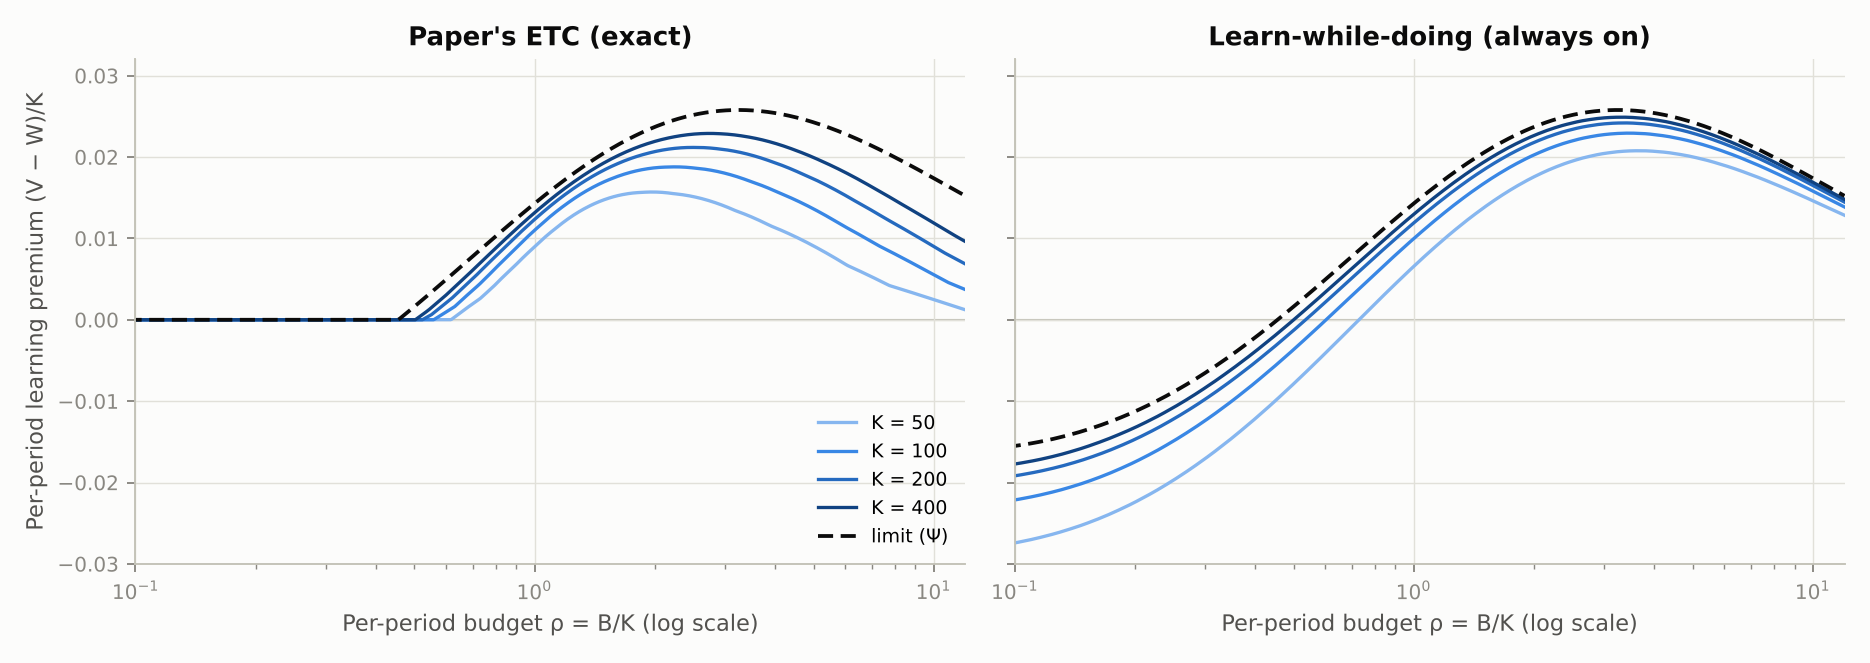
\includegraphics[width=\textwidth]{figs/fig_premium_convergence.png}
\caption{Per-period learning premium for $K=50,100,200,400$ (light to dark) and the limit (dashed). Left: the paper's
ETC converges to $\Psi=\max\{\VPI,0\}$. Right: a learn-while-doing team converges to $\VPI$, which is negative below
$\rho_1$ (free information lowers the value of a budget-paced team).}
\label{fig:conv}
\end{figure}

\paragraph{Allocation.} Table~\ref{tab:switch} reports the total budget per period $t=T/K$ at which learning first
moves the split (toward the senior team) and at which the shift turns negative (toward the junior team). Both
switch points converge to the same limit for the two protocols, as Corollary~\ref{cor:alloc} predicts; at the limit
switch $t=1.5$ the junior team's benchmark budget per period is $\approx0.48$, just above $\rho_1$. The CE team's
normalised shift converges quickly (e.g.\ $-0.0329,-0.0319,-0.0315,-0.0314$ at $t=2.5$, limit $-0.0311$); the ETC
team's converges more slowly, and its finite-$K$ ``re-concentration'' at large $t$ moves to ever larger budgets
(Figure~\ref{fig:alloc}), consistent with Proposition~\ref{prop:shape}(c).

\begin{table}[h]
\centering\small
\caption{Switch points of the allocation shift $(a^L_K-a^E_K)/K$ in $t=T/K$ ($v_1/v_2=2$).}
\label{tab:switch}
\begin{tabular}{@{}lccccc@{}}
\toprule
& $K=50$ & $K=100$ & $K=200$ & $K=400$ & limit\\
\midrule
ETC: shift becomes positive & 0.90 & 0.85 & 0.80 & 0.75 & 0.65\\
ETC: shift turns negative & 1.95 & 1.85--1.95 & 1.75 & 1.65--1.70 & 1.50\\
CE: shift becomes positive & 1.05 & 0.90 & 0.80 & 0.75 & 0.65\\
CE: shift turns negative & 2.30 & 1.95 & 1.75 & 1.65 & 1.50\\
\bottomrule
\end{tabular}
\end{table}

\begin{figure}[h]
\centering
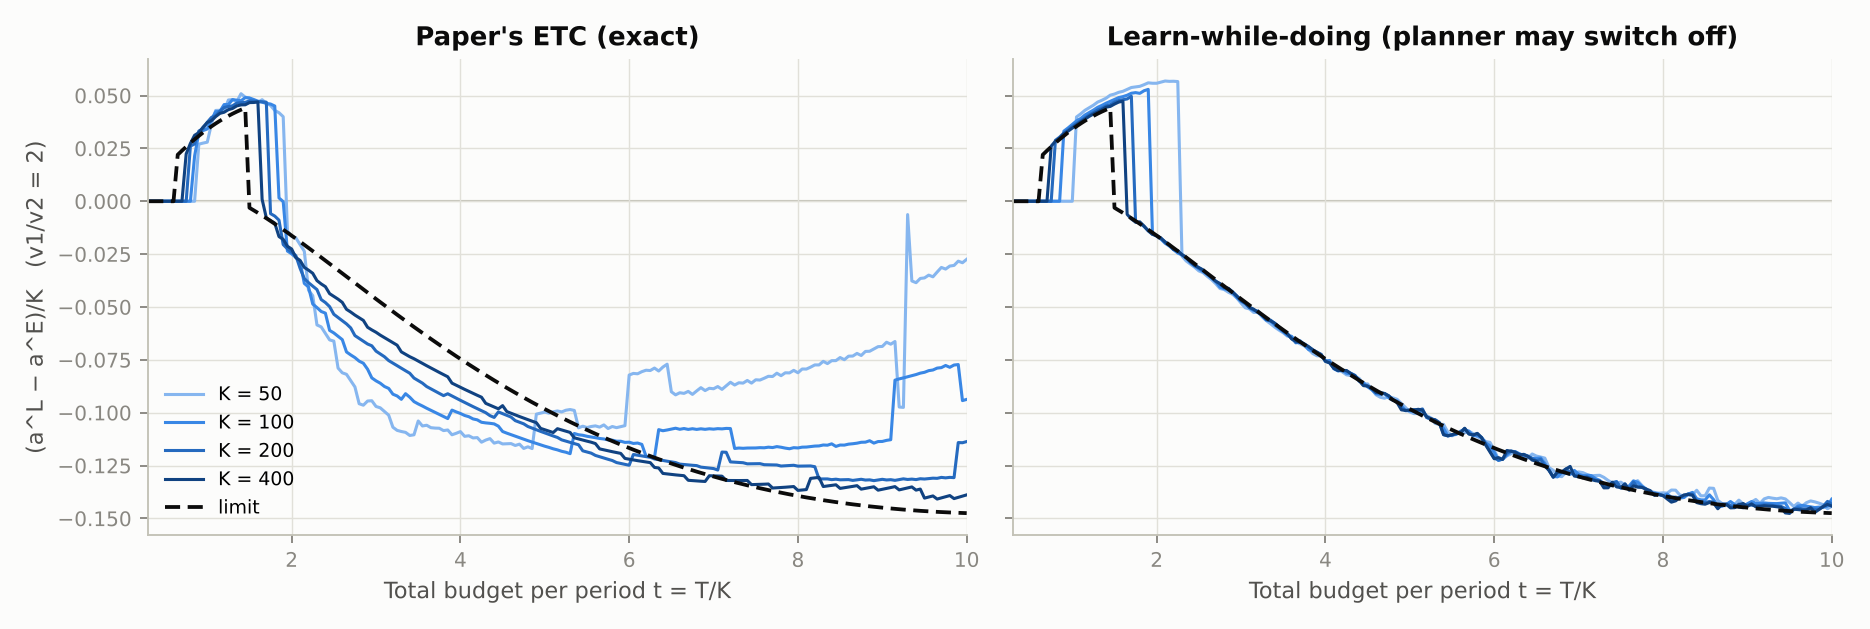
\includegraphics[width=\textwidth]{figs/fig_allocation_convergence.png}
\caption{Normalised allocation shift $(a^L_K-a^E_K)/K$ for $K=50,100,200,400$ and the limit of
Corollary~\ref{cor:alloc} (dashed). Both protocols converge to the same limit.}
\label{fig:alloc}
\end{figure}

\paragraph{Open points.} (i) Uniqueness of the zero of $\VPI$ and transversality at entry are verified numerically
here and across the parameter sweep, but not proved. (ii) A proof of the CE limit. (iii) A probing design that
implements the concave envelope (e.g.\ a planner-chosen probe bid with belief-dependent stopping) would lower the
limit entry point from $\rho_1=0.456$ toward $0.305$; Proposition~\ref{prop:limit}(b) shows that no learn-then-commit
protocol can do better than $\Phi$.

\end{document}
